%!TEX root = ../bericht.tex

\section{Einleitung}

eee

\section{Methoden}


	\subsection{Konzept}
	
		In der Entwicklung einer Osteosyntheseplatte sollen unterschiedliche Aspekte.
		Darunter fallen folgende Aspekte:
		
		\begin{enumerate}
			\setlength{\itemsep}{0mm}
			\setlength{\parskip}{1mm}
			\item Möglichst Minimal-Invasive Technik um Weichteile nicht zu verletzen
		\end{enumerate}
		
		Da meine CAD Konstruktions-Fähigkeiten beschränkt sind 	
		

\section{CAD Modellierung}

\section{FEM Analyse}

	\subsection{Materialdaten}
		\begin{center}
			\begin{tabular}{ | p{6cm} | p{3cm} | }
				\multicolumn{1}{l}{\bfseries Material} & \multicolumn{1}{l}{\bfseries E-Modus } \\ \hline
				Knochen (bone) & $ 1300 \frac{kg}{m^3} $ \\ \hline
				Titanlegierung (titanium alloy) & $ 4620 \frac{kg}{m^3} $ \\ \hline
			\end{tabular}
			\captionof{table}{Materialdaten}
			\label{fig:device3}
		\end{center}

	\subsection{Vernetzung}
		\begin{Figure}
			\centering
			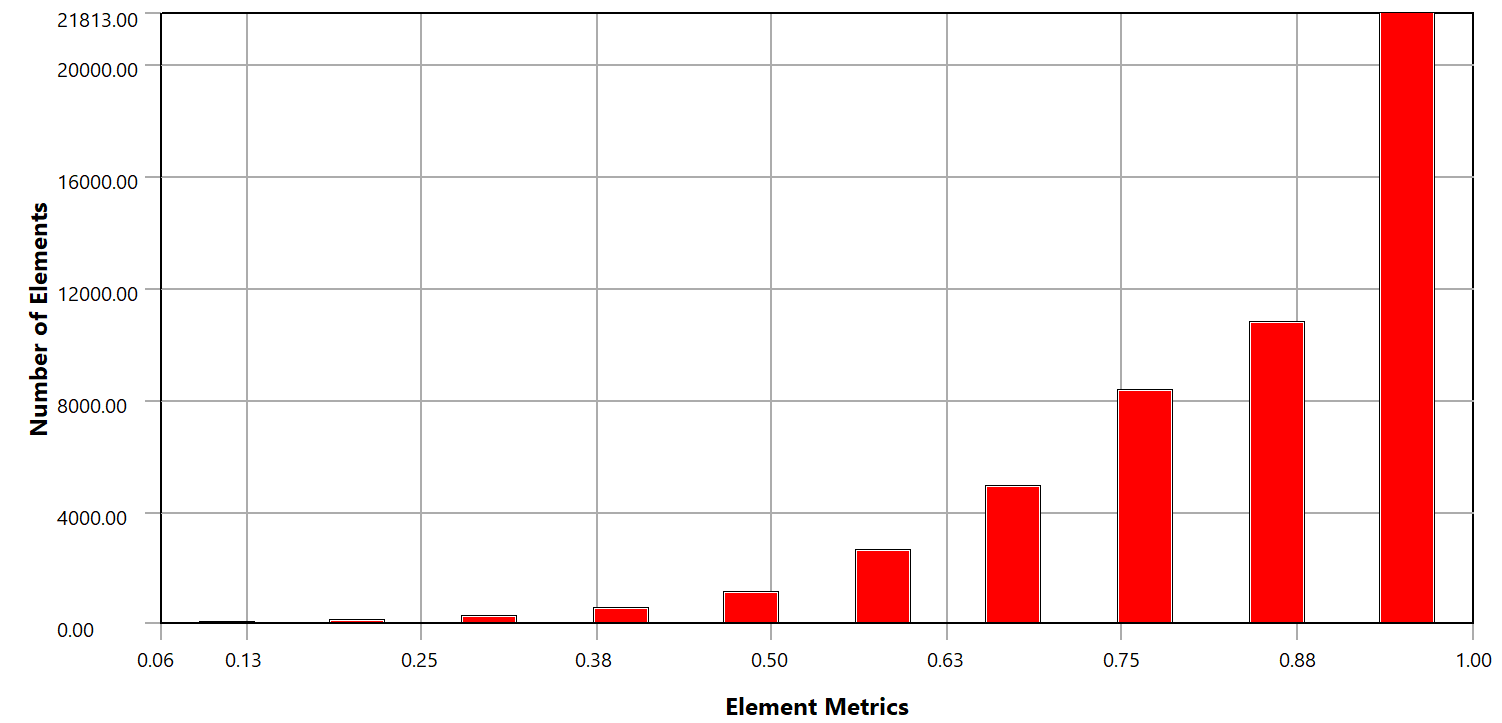
\includegraphics[width=15cm]{content/images/mesh_quality.png}
			\captionof{figure}{Magic-Angle-Spinning (MAS) Aufbau}
			\label{fig:device3}
		\end{Figure}
		
		\begin{Figure}
			\centering
			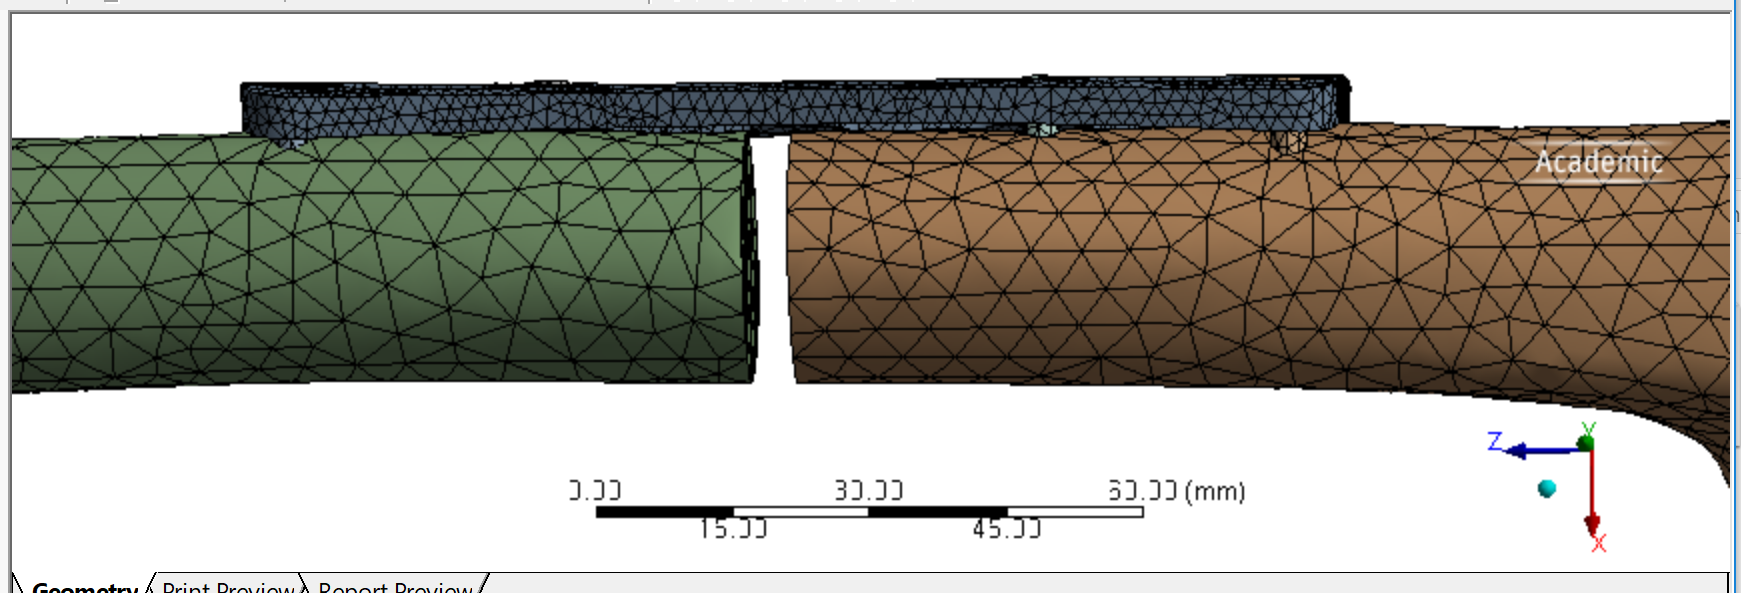
\includegraphics[width=15cm]{content/images/mesh_quality_graph_2.png}
			\captionof{figure}{Magic-Angle-Spinning (MAS) Aufbau}
			\label{fig:device3}
		\end{Figure}
		
		\begin{Figure}
			\centering
			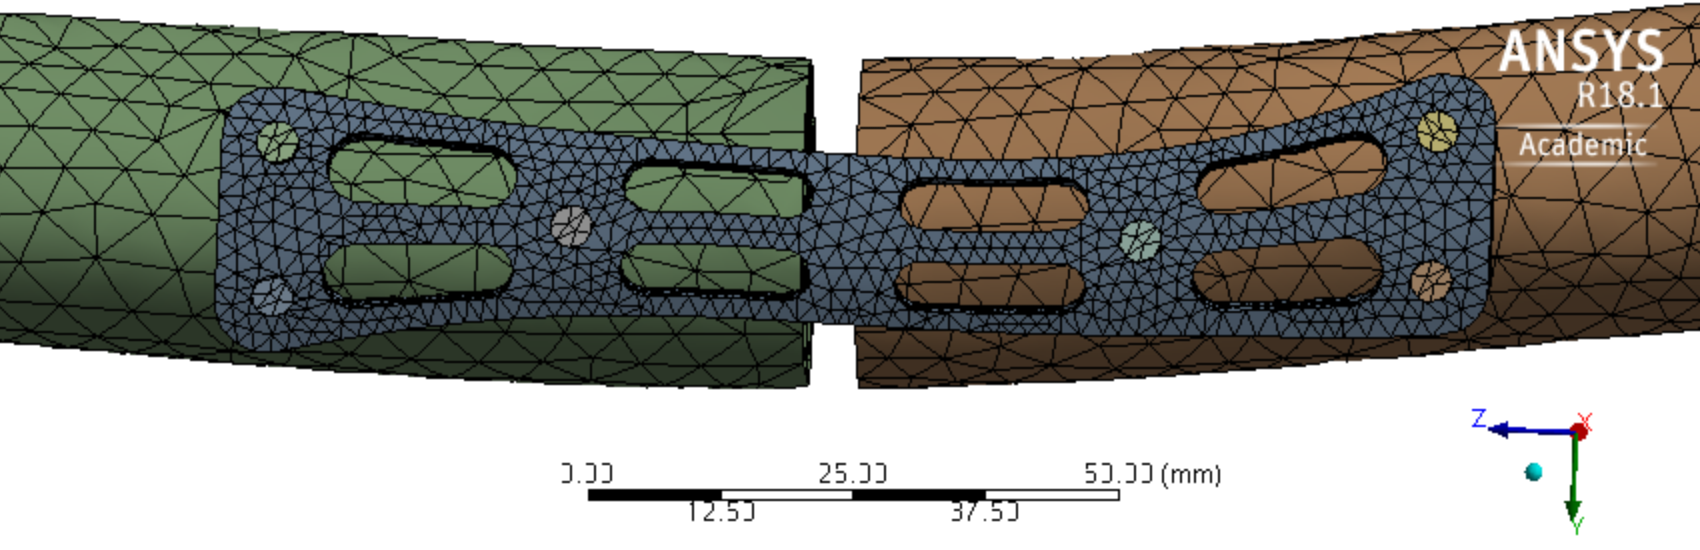
\includegraphics[width=15cm]{content/images/mesh_quality_graph_3.png}
			\captionof{figure}{Magic-Angle-Spinning (MAS) Aufbau}
			\label{fig:device3}
		\end{Figure}

	\subsection{Lager- und Reaktionskräfte}
		\begin{Figure}
			\centering
			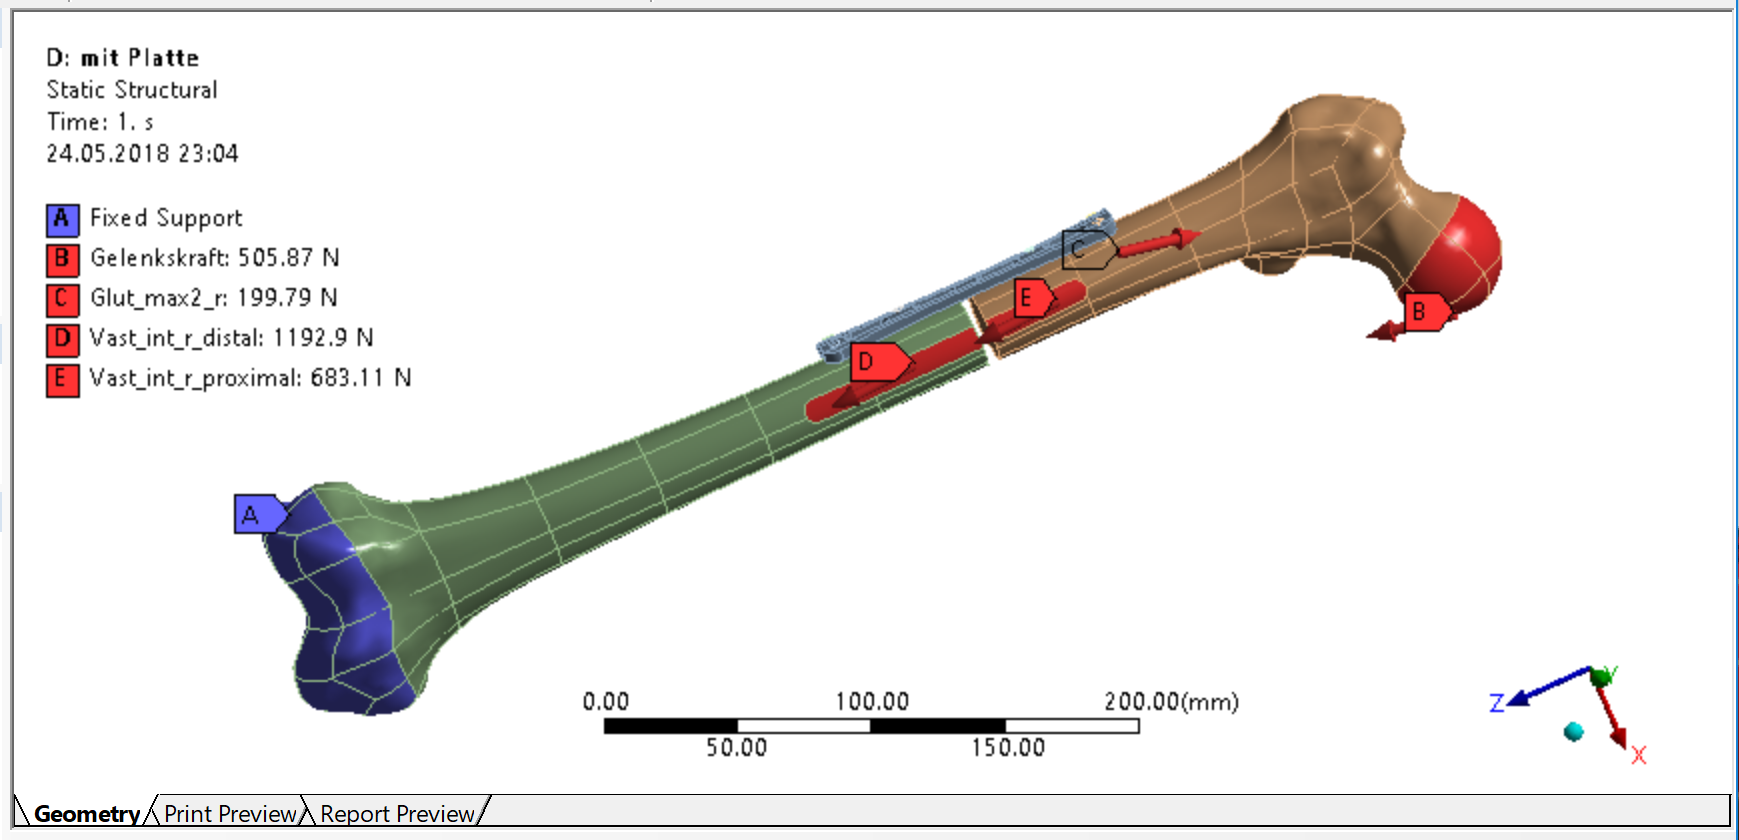
\includegraphics[width=15cm]{content/images/kraefte.png}
			\captionof{figure}{Magic-Angle-Spinning (MAS) Aufbau}
			\label{fig:device3}
		\end{Figure}


\section{Resultate}

	\subsection{Gesamtverformung}
	
		\begin{Figure}
			\centering
			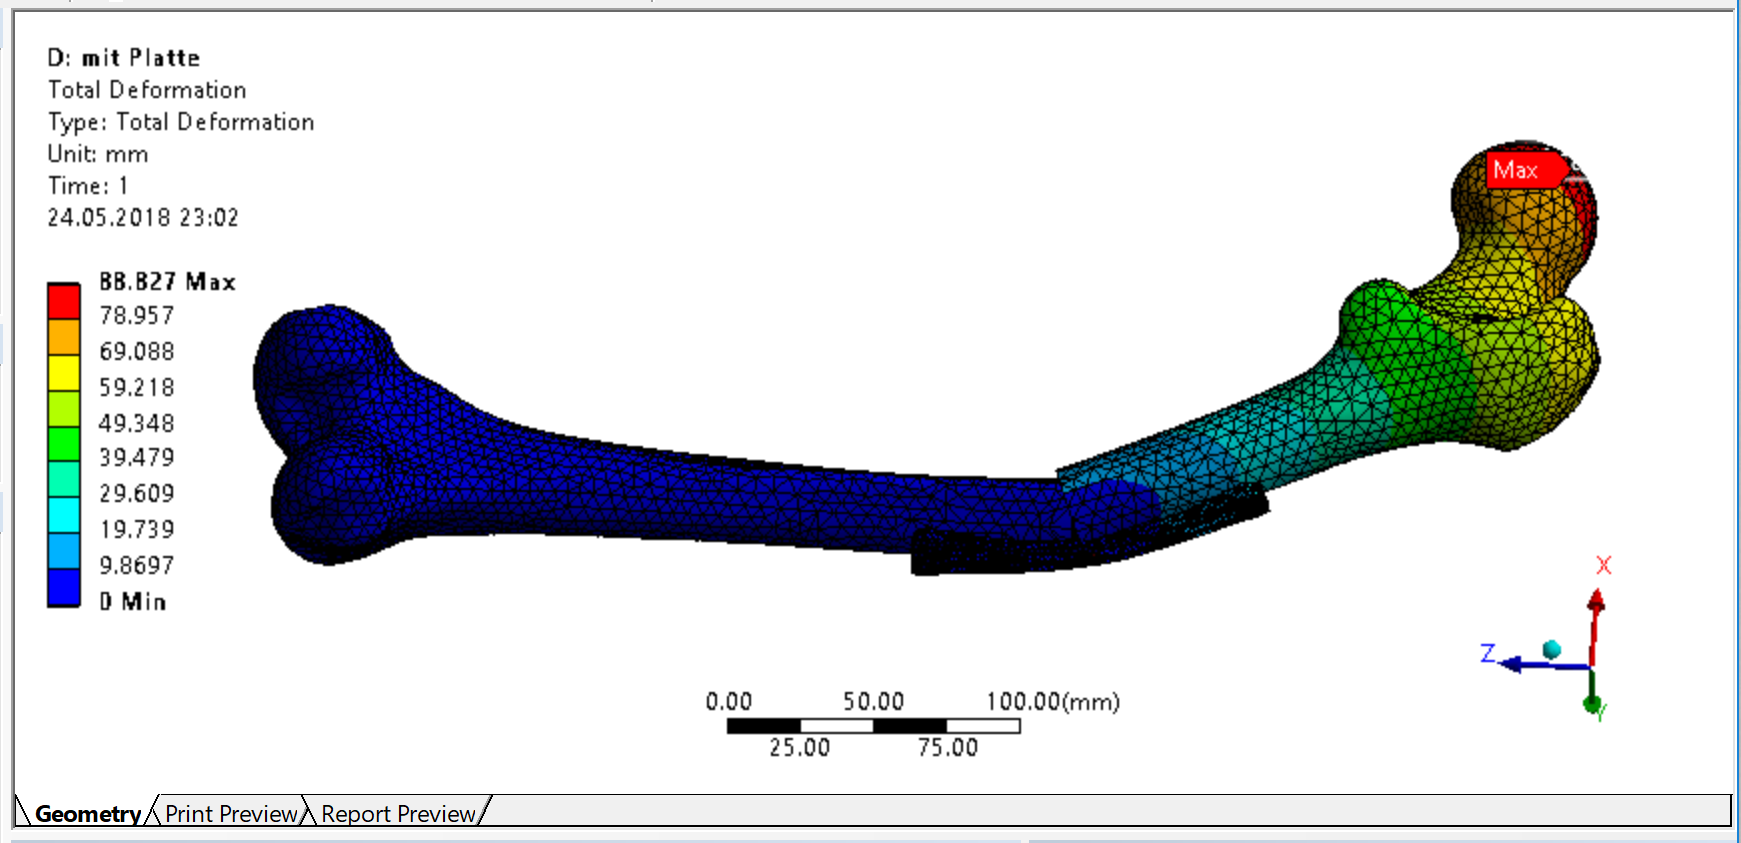
\includegraphics[width=15cm]{content/images/deformation.png}
				\captionof{figure}{Gesamtdeformation der Osteosyntheseplatte}
			\label{fig:deformation}
		\end{Figure}
	
		\subsubsection{Vergleichsplatte}
	
			\begin{Figure}
				\centering
				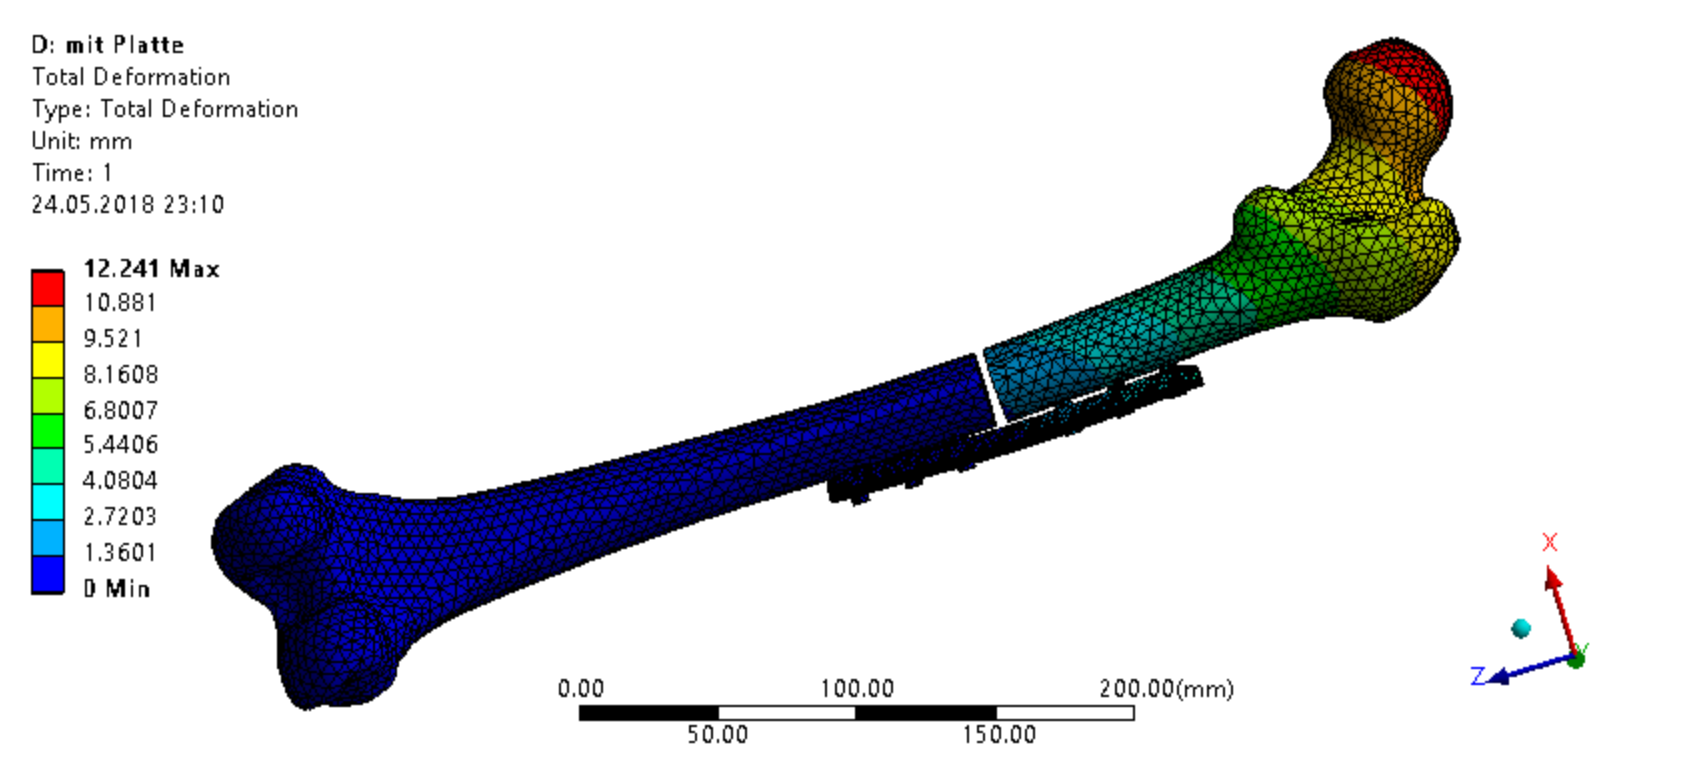
\includegraphics[width=15cm]{content/images/vergleich_deformation.png}
				\captionof{figure}{Gesamtdeformation der Vergleichsplatte}
				\label{fig:vergleich_deformation}
			\end{Figure}
	
	\subsection{Vergleichsspannung}
	
		\begin{Figure}
			\centering
			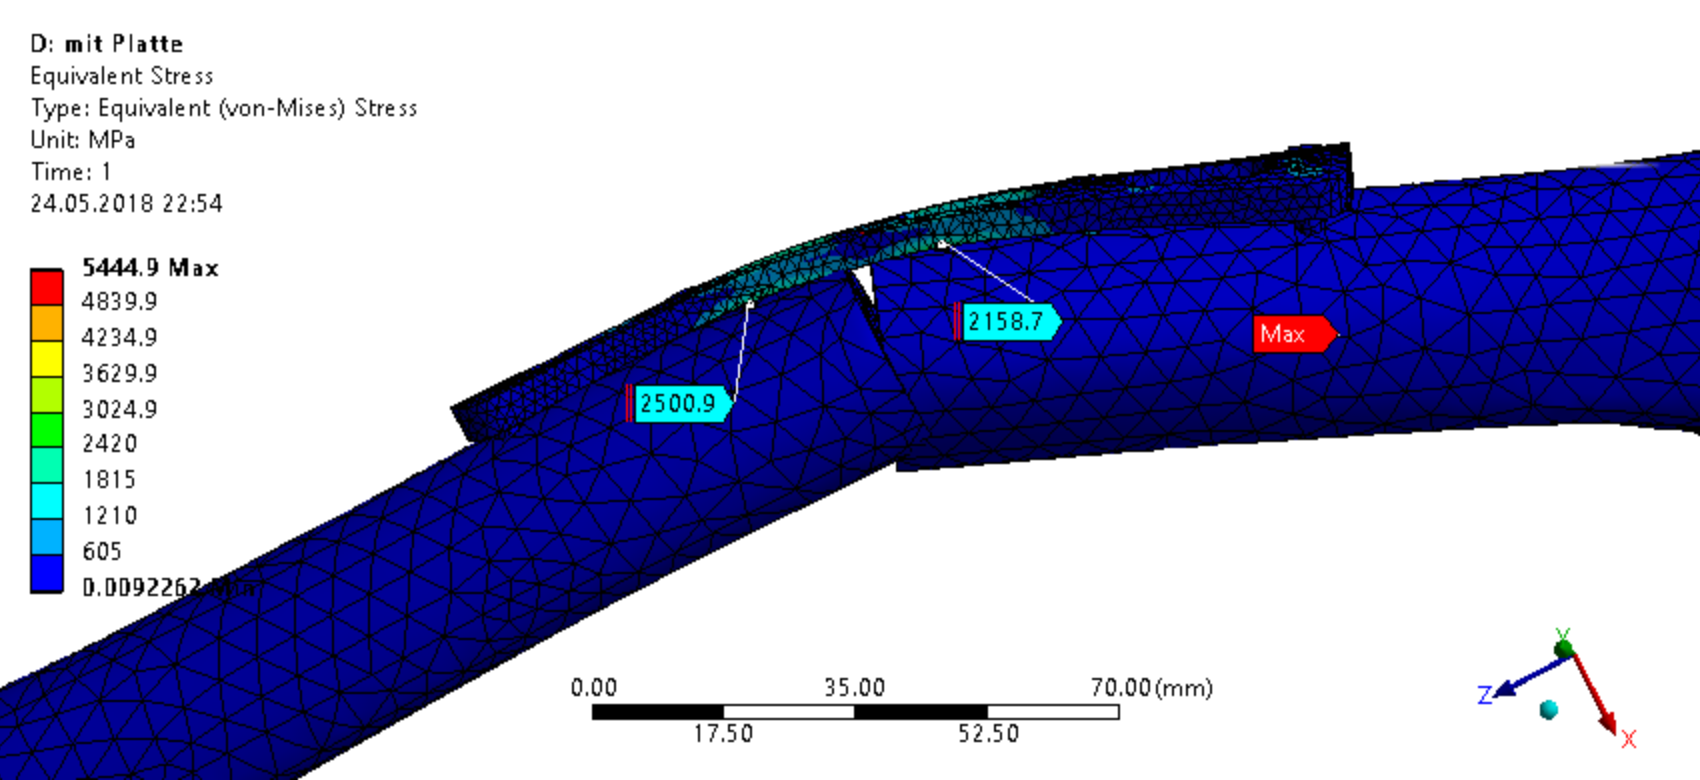
\includegraphics[width=15cm]{content/images/stress_side.png}
			\captionof{figure}{Vergleichsspannung der Osteosyntheseplatte (vorne)}
			\label{fig:stress_side}
		\end{Figure}
	
		\begin{Figure}
			\centering
			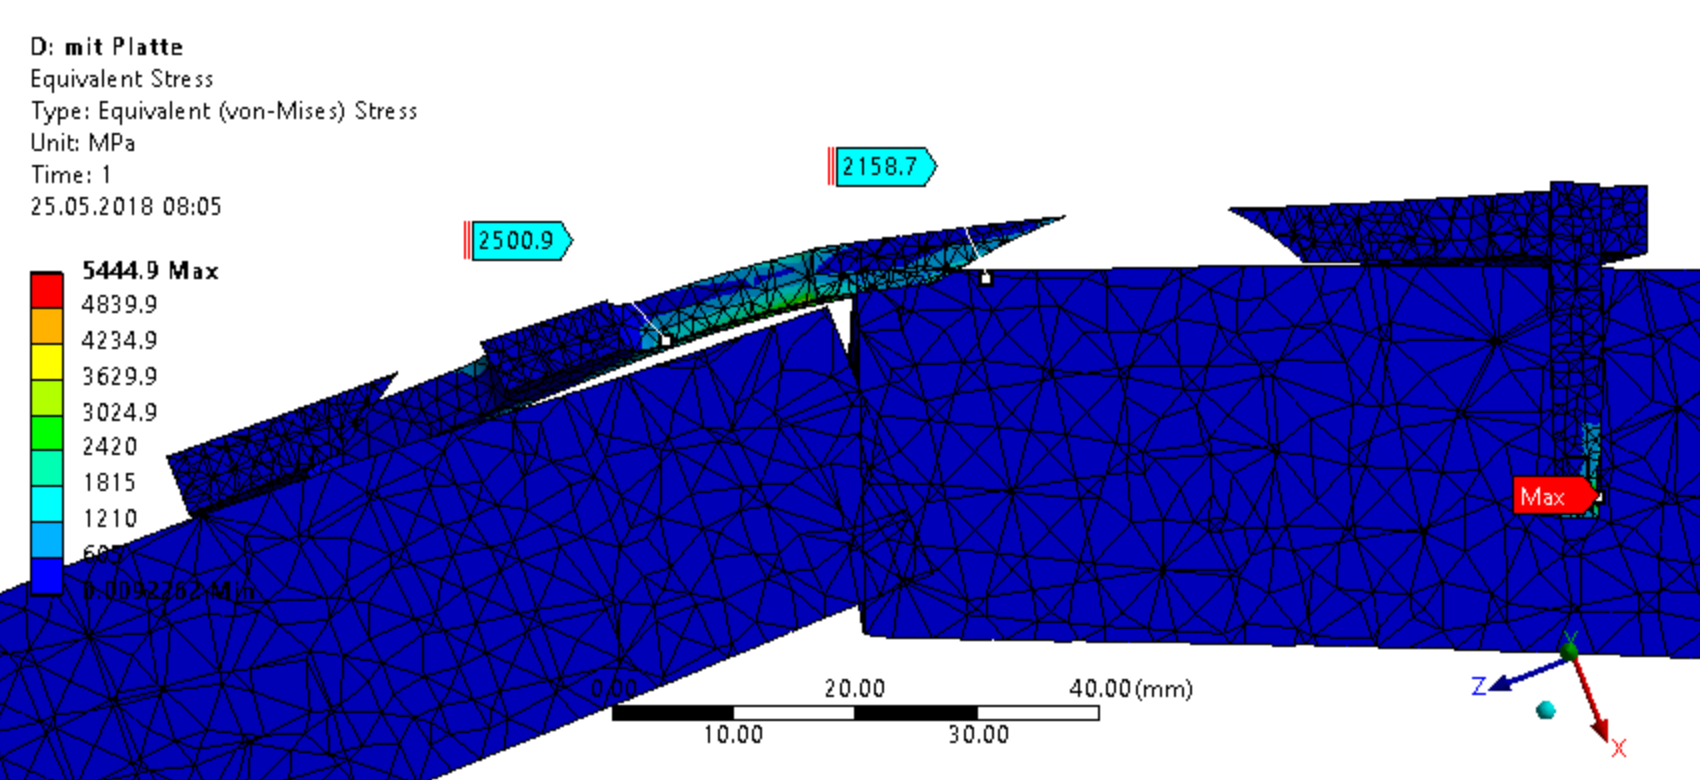
\includegraphics[width=15cm]{content/images/stress_side_profile.png}
			\captionof{figure}{Vergleichsspannung der Osteosyntheseplatte (vorne, im Querschnitt)}
			\label{fig:stress_side_profile}
		\end{Figure}
	
		\begin{Figure}
			\centering
			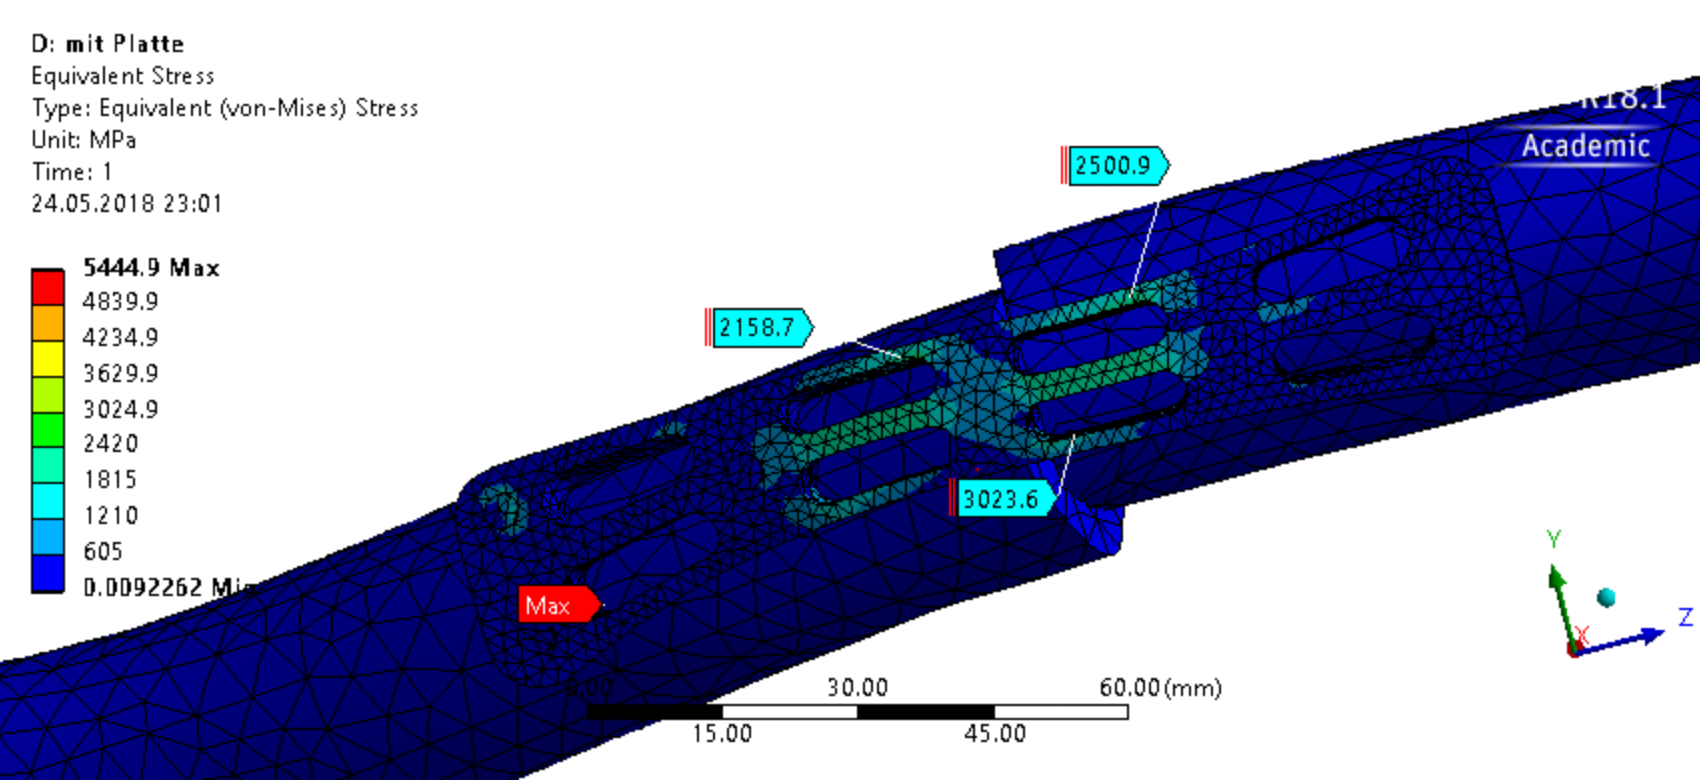
\includegraphics[width=15cm]{content/images/stress_top.png}
			\captionof{figure}{Vergleichsspannung der Osteosyntheseplatte (oben)}
			\label{fig:stress_top}
		\end{Figure}
		
		\subsubsection{Vergleichsplatte}
		
			\begin{Figure}
				\centering
				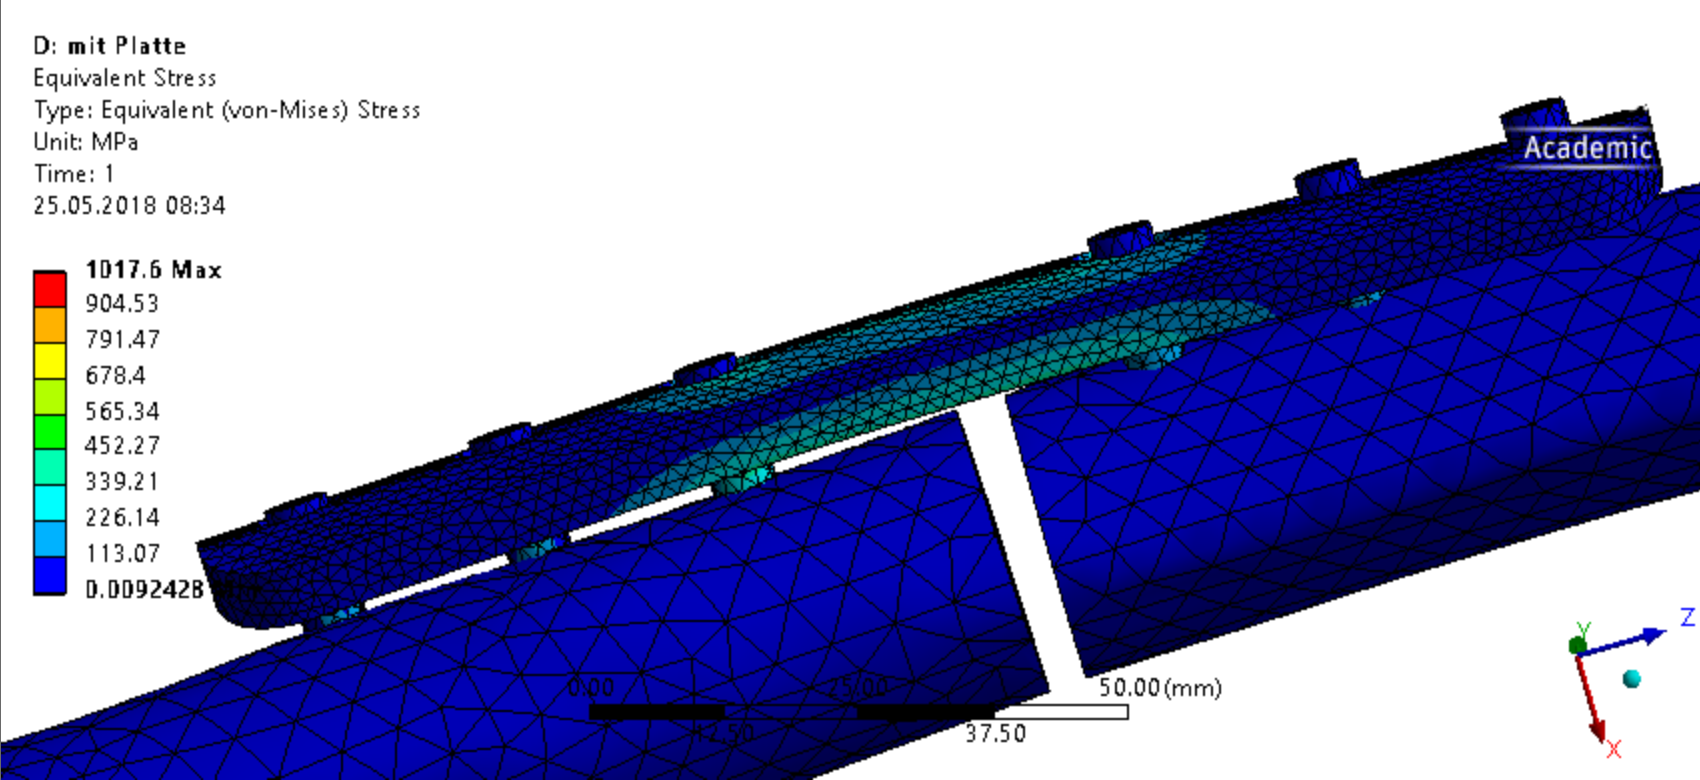
\includegraphics[width=15cm]{content/images/vergleich_stress_side.png}
				\captionof{figure}{Vergleichsspannung der Vergleichsplatte (vorne)}
				\label{fig:vergleich_stress_side}
			\end{Figure}
		
			\begin{Figure}
				\centering
				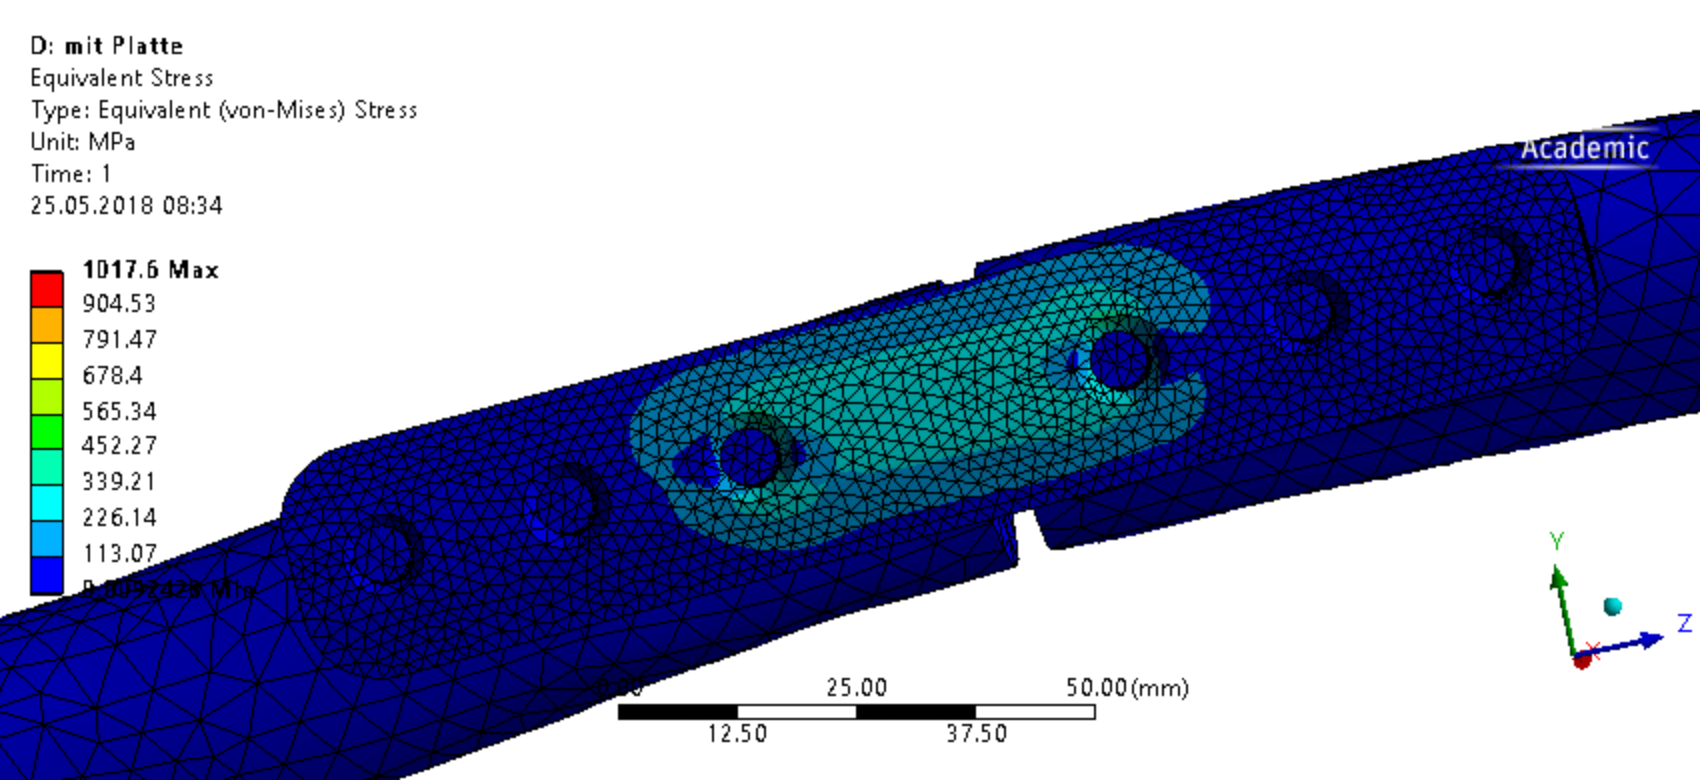
\includegraphics[width=15cm]{content/images/vergleich_stress_top.png}
				\captionof{figure}{Vergleichsspannung der Vergleichsplatte (oben)}
				\label{fig:vergleich_stress_top}
			\end{Figure}
	
	


\section{Diskussion}

	ccc

